\chapter{Охрана труда и окружающей среды}
\section{Анализ условий труда}
\subsection{Обеспечение условий труда в отделе разработки программного обеспечения}
Дипломная работа посвящена разработке системы мониторинга состояния ЛА на основе алгоритмов интеллектуального анализа данных. Разработка производится на персональном компьютере и предполагает длительное пребывание за ним инженера.

Применение персонального компьютера освобождает человека от непроизводительной работы, связанной с обработкой информации, изменяет характер его труда. Однако при этом увеличивается доля умственного и нервно-напряженного труда, возрастает психоэмоциональная нагрузка. При значительной трудовой нагрузке, нерациональной организации работы и неблагоприятных факторах производственной среды быстро снижается работоспособность операторов, уменьшается производительность труда и ухудшается качество работы, может развиться перенапряжение,~а в отдельных случаях возникнуть срыв трудовой деятельности~— дистресс.

В данном разделе проводится анализ условий труда в отделе разработки информационных систем с целью обеспечения безопасности и удобства, требуемых для работы инженера.

\subsection{Характеристика помещения}
Помещение находится в здании Московского Авиационного Института и представляет собой кафедральную лабораторию со следующими параметрами:
%\begin{itemize}
\begin{enumerate}
\item длина~6~м;
\item ширина~4~м;
	\begin{enumerate}
	\item трампампам
	\item тарарам
	\end{enumerate}
\item высота~3,5~м.
%\end{itemize}
\end{enumerate}

Общая площадь: $6\times4 = 24$~м\textsuperscript{2}.

Объём: $6\times4\times3,5 = 84$~м\textsuperscript{3}.

Количество рабочих мест~—~4.

Количество одновременно находящихся в помещении сотрудников не превышает~4 человек.

План помещения приведён на рисунке~\ref{image:room_plan}.
\begin{figure}[h]
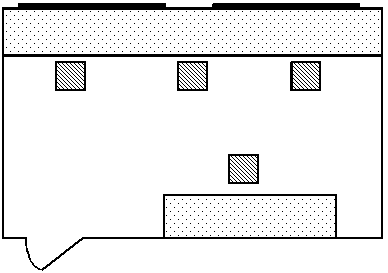
\includegraphics[width=0.6\textwidth, keepaspectratio]{plan}
\caption{План помещения}\label{image:room_plan}
\end{figure}